%------------------------------------------------------------------------
%Editar Diplomado
\hypertarget{cv:eliminarTray}{\section{Eliminar Trayectoria}} \label{sec:eliminarTray}

	Esta funcionalidad le permitirá eliminar una trayectoria innecesaria o incorrecta. Para eliminar una trayectoria es necesario que no se encuentre asociada en otros casos de uso.

		\subsection{Procedimiento}

			%Pasos de procedimiento
			\begin{enumerate}
	
			\item Oprima el botón \IUBotonEliminar{} de un registro existente de la pantalla \ref{fig:GestionarTrayectorias} ''Gestionar Trayectorias''.
	
			\item Se mostrará el mensaje \ref{fig:confirmaEliminaTray} sobre la pantalla \ref{fig:GestionarTrayectorias} ''Gestionar Trayectorias''.
			
			%Pantalla
			\begin{figure}[htbp!]
				\begin{center}
					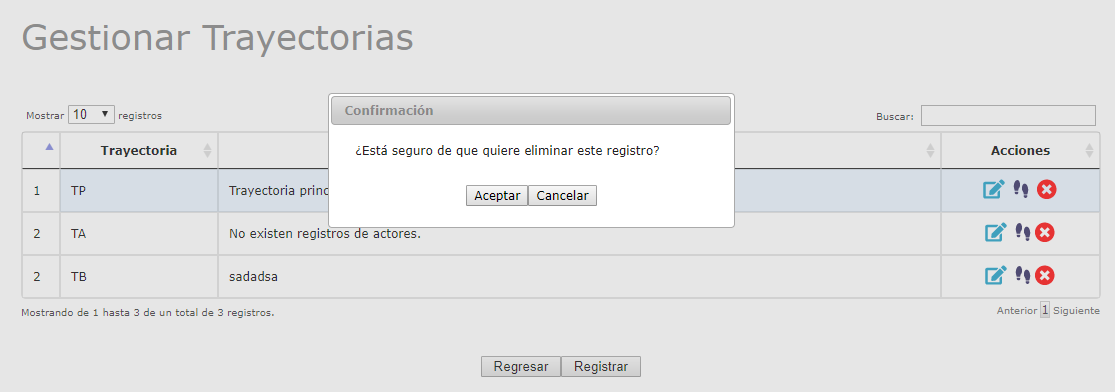
\includegraphics[scale=0.6]{roles/lider/casosUso/trayectorias/pantallas/IU6-1-1-3MSG10}
					\caption{MSG de Confirmación}
					\label{fig:confirmaEliminaTray}
				\end{center}
			\end{figure}
						
			\item Oprima el botón \IUAceptar.
			
			\item Se mostrará el mensaje \ref{fig:trayEliminada} en la pantalla \ref{fig:GestionarTrayectorias} ''Gestionar Trayectorias''.
			
			\begin{figure}[htbp!]
				\begin{center}
					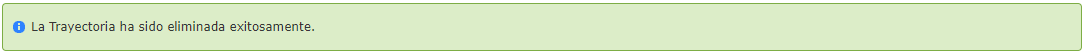
\includegraphics[scale=0.6]{roles/lider/casosUso/trayectorias/pantallas/IU6-1-1-3MSG1}
					\caption{MSG: Trayectoria Eliminada}
					\label{fig:trayEliminada}
				\end{center}
			\end{figure}
			\end{enumerate}